\section{Deadlock BPaxos}\appendixlabel{DeadlockBPaxosAppendix}
\subsection{Pruned Dependencies}
Here, we prove that \invref{DependencyService} and \invref{PrunedDependencies}
imply \invref{ConflictInvariant}.
%
Consider two conflicting commands $x$ and $y$ chosen in instances $I_x$ and
$I_y$. $x$ and $y$ conflict, so neither is $\noop$. Thus, by
\invref{PrunedDependencies}, $I_x$ is chosen with pruned dependencies
$\deps{I_x} - P_x$ and $I_y$ is chosen with pruned dependencies $\deps{I_y} -
P_y$ derived from dependencies $\deps{I_x}$ and $\deps{I_y}$ computed by the
dependency service. We want to show that $I_x \in \deps{I_y} - P_y$ or $I_y \in
\deps{I_x} - P_x$, or both.
%
By \invref{DependencyService}, either $I_y \in \deps{I_x}$ or $I_x \in
\deps{I_y}$ or both. Without loss of generality, assume $I_y \in \deps{I_x}$.
If $I_y$ is also in $\deps{I_x} - P_x$, then we're done. Otherwise, $I_y$ has
been pruned from $\deps{I_x}$ (i.e.\ $I_y \in P_x$). This happens only if $y$
is a $\noop$ or if $I_y$ has been chosen with $I_x \in \deps{I_y} - P_y$. $y$
is not a $\noop$, so $I_x \in \deps{I_y} - P_y$.

\subsection{Deadlock Example}
Consider a Deadlock BPaxos deployment with $n = 9$ dependency service nodes
(i.e., $f = 4$). Imagine four of these nodes have failed. The conflict graphs
of the remaining five ordering service nodes are illustrated in
\figref{DeadlockBPaxosExample}. All five dependency service nodes have
processed five commands $x_0$ through $x_4$ in instances $I_0$ through $I_4$
respectively. Every command $x_i$ conflicts with $x_{i - 1 \bmod 5}$ and $x_{i
+ 1 \bmod 5}$. For example, $x_0$ conflicts with $x_4$ and $x_1$. Dependency
service node $d_1$ has processed the five commands in the order $x_0, x_1, x_2,
x_3, x_4$, dependency service node $d_2$ has processed the five commands in the
order $x_1, x_2, x_3, x_4, x_0$, and so on.

{

\begin{figure}[ht]
  \centering

  \tikzstyle{smallsquare}=[
    draw,
    line width=1pt,
    minimum height=0.25in,
    minimum width=0.25in,
  ]

  \tikzstyle{dep}=[
    -latex,
    ultra thick,
  ]

  \begin{subfigure}[b]{0.3\textwidth}
    \centering
    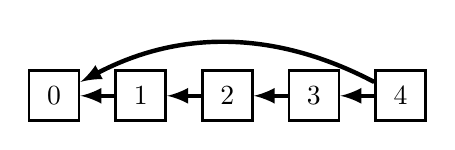
\begin{tikzpicture}[xscale=1.1]
      \foreach \i [count=\x] in {0, 1, 2, 3, 4} {%
        \node[smallsquare] (\i) at (\x, 0) {$\i$};
      }
      \draw[dep] (1) to (0);
      \draw[dep] (2) to (1);
      \draw[dep] (3) to (2);
      \draw[dep, bend right] (4) to (0);
      \draw[dep] (4) to (3);
    \end{tikzpicture}
    \caption{$G_1$}\figlabel{DeadlockBPaxosExampleG1}
  \end{subfigure}
  \hspace{1in}%
  \begin{subfigure}[b]{0.3\textwidth}
    \centering
    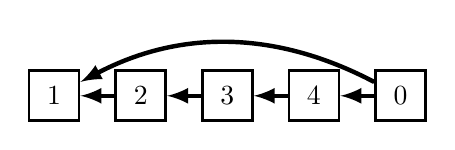
\begin{tikzpicture}[xscale=1.1]
      \foreach \i [count=\x] in {1, 2, 3, 4, 0} {%
        \node[smallsquare] (\i) at (\x, 0) {$\i$};
      }
      \draw[dep, bend right] (0) to (1);
      \draw[dep] (0) to (4);
      \draw[dep] (2) to (1);
      \draw[dep] (3) to (2);
      \draw[dep] (4) to (3);
    \end{tikzpicture}
    \caption{$G_2$}\figlabel{DeadlockBPaxosExampleG2}
  \end{subfigure}

  \vspace{0.2in}

  \begin{subfigure}[b]{0.3\textwidth}
    \centering
    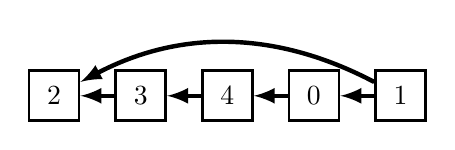
\begin{tikzpicture}[xscale=1.1]
      \foreach \i [count=\x] in {2, 3, 4, 0, 1} {%
        \node[smallsquare] (\i) at (\x, 0) {$\i$};
      }
      \draw[dep] (0) to (4);
      \draw[dep] (1) to (0);
      \draw[dep, bend right] (1) to (2);
      \draw[dep] (3) to (2);
      \draw[dep] (4) to (3);
    \end{tikzpicture}
    \caption{$G_3$}\figlabel{DeadlockBPaxosExampleG3}
  \end{subfigure}
  \hspace{1in}%
  \begin{subfigure}[b]{0.3\textwidth}
    \centering
    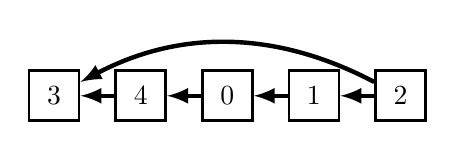
\begin{tikzpicture}[xscale=1.1]
      \foreach \i [count=\x] in {3, 4, 0, 1, 2} {%
        \node[smallsquare] (\i) at (\x, 0) {$\i$};
      }
      \draw[dep] (0) to (4);
      \draw[dep] (1) to (0);
      \draw[dep] (2) to (1);
      \draw[dep, bend right] (2) to (3);
      \draw[dep] (4) to (3);
    \end{tikzpicture}
    \caption{$G_4$}\figlabel{DeadlockBPaxosExampleG4}
  \end{subfigure}

  \vspace{0.2in}

  \begin{subfigure}[b]{0.3\textwidth}
    \centering
    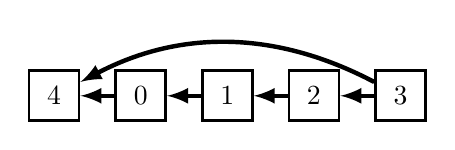
\begin{tikzpicture}[xscale=1.1]
      \foreach \i [count=\x] in {4, 0, 1, 2, 3} {%
        \node[smallsquare] (\i) at (\x, 0) {$\i$};
      }
      \draw[dep] (0) to (4);
      \draw[dep] (1) to (0);
      \draw[dep] (2) to (1);
      \draw[dep] (3) to (2);
      \draw[dep, bend right] (3) to (4);
    \end{tikzpicture}
    \caption{$G_5$}\figlabel{DeadlockBPaxosExampleG5}
  \end{subfigure}

  \caption{A Deadlock BPaxos deadlock}%
  \figlabel{DeadlockBPaxosExample}
\end{figure}
}

Imagine Deadlock BPaxos node $b_i$ attempts to recover instance $I_0$.
$\QuorumMajoritySize$ acceptors have voted for $\deps{x_0} = \set{x_4}$, but
$d_2$ voted for $\set{x_1, x_4}$. Thus, $b_i$ attempts to recover $I_1$.
$\QuorumMajoritySize$ acceptors have voted for $\deps{x_1} = \set{x_0}$, but
$d_3$ voted for $\set{x_0, x_2}$, so $b_i$ attempts to recover $I_2$. This
continues until $b_i$ attempts to recover $I_4$.  $\QuorumMajoritySize$
acceptors have voted for $\deps{x_4} = \set{x_3}$, but $d_1$ voted for
$\set{x_0, x_3}$, so $b_i$ attempts to recover $I_0$. This is a deadlock.
